\section{Laboratory work implementation}

\subsection{Tasks and Points}

\begin{itemize}
	\item Aplicatia trebuie sa fie dezvoltata si testata cu orice SDK ce include Emulator
	\item Testarea aplicatiei pe un device real
	\item Aplicatia trebuie sa suporte device-urile cu diferite rezolutii
	\item O alta aplicatie sofisticata la alegere: Game
	\item Foloseste libraria cross platform pentru a realiza o apliacatie cross platform (aplicatia poate fi compilata atit pe Android, cit si pe iOS)
\end{itemize}

\subsection{Analiza lucrarii de laborator}
Repository \href{https://github.com/AScripnic/MIDPS-laboratories/tree/master/Lab%234}{link}\par

Primul pas spre elaborarea jocului a fost studiere api-ului de bază a IDE-ului Unity și lucrul cu scena de bază a lui \cite{unity}. Pentru început am studiat GameObjects și metoda de a manipula Componentele lui de gen Transform, Rigidbody2D, BoxCollider2D, etc.

Al doilea pas a fost deciderea jocului și tema lui. După navigarea mai detaliată pe GooglePlay am decis să creez un Endless Runner, care este mai simplu pentru un începător și e mai ușor la generarea nivelului.

Prima problemă întâlnită în joc a fost metoda de miscare a nivelului și mai precis:

\begin{enumerate}
	\item Personajul va sta pe loc, iar restul nivelului se va mișca, iar personajul principal va sta pe loc.
	\item Personajul va sta pe loc, iar restul nivelului nu se va mișca
\end{enumerate}

Ambele au si pro și con, ca exemplu varianta a ne dă voie să nu simulăm aplicarea forțelor asupra personajului și con că trebuie să mișcăm tot nivelul și inclusiv obiectele generate dynamic. După studirerea a mai multor tutoriale\cite{endless-runner-force}, am decis să mă țin de varianta (b). 

Al treilea pas a fost de a crea obiecte de bază, Sprites, care seminificau Player, Obstacles, Ground. Primul \href{https://github.com/AScripnic/MIDPS-laboratories/blob/master/Lab%234/Running%20Man/Assets/PlayerBehaivor.cs}{script}\cite{scripting} creat a fost pentru Player care aplică o viteză de mișcare asupra obiectului(Rigidbody2D) ce îl reprezintă pentru a se misca pe elementul Ground. Apoi am creat un punct invizibil care prin intermediul unui \href{https://github.com/AScripnic/MIDPS-laboratories/blob/master/Lab%234/Running%20Man/Assets/GroundGenerator.cs}{script} determină daca trebuie mutată copia elementul\cite{instantiate} Ground în fața jucătorului pentru a crea o iluzie că pământul nu este finit.

Al patrulea pas a constituit în crearea \href{https://github.com/AScripnic/MIDPS-laboratories/blob/master/Lab%234/Running%20Man/Assets/ObstaclesGenerator.cs}{a scriptului} ce genera dinamic obstacolele de care personajul ar trebui să se ferească.

După finisarea mecanicii jocului, jucătorul avea posibilitatea de a face 3 acțiuni:
\begin{itemize}
	\item Run - Stare de bază a jucătorului este de a fugi
	\item Jump - Personajul sare peste obstacole
	\item Slide - Personajul se lușuie sub obstacole
\end{itemize}

Următorul pas constă în adăugarea texturilor și animațiilor necesare pentru finisarea jocului. Pentru jucător am implementat 1 textură și 4 animații\cite{animation}: Run, Jump, Slide, Lose
\begin{itemize}
	\item Run \ref{run}
	\item Jump \ref{jump}
	\item Slide \ref{slide}
	\item Lose \ref{lose}
\end{itemize}

În urma animației Slide am fost nevoit să editez dynamic zona de impact cu alte obiecte (BoxCollider2D) asa cum poziția lui se schimbă.

Pentru obstacole a fost mai greu, deoarece am fost nevoit sa le editez manual pe fiecare în parte și modificare cu obiectul original, care era doar un dreptunghi, și editarea zonei de impact cu utilizatorul (BoxCollider2D). Texturile pentru Ground a fost mai ușor de găsit așa cum este mai des folosite în diferite jocuri, dar versiunea current de Unity nu permite repetarea unui texture pe zona lui de mai multe ori, și am fost nevoit să creez o textură de dimensiunea exactă la Ground.

Ultemele detalii în crearea jocului a fost adăugarea scorului și testarea aplicației pe un dispozitiv mobil.


\subsection{Imagini}
\begin{center}
	\begin{figure}[h]
		\centering
		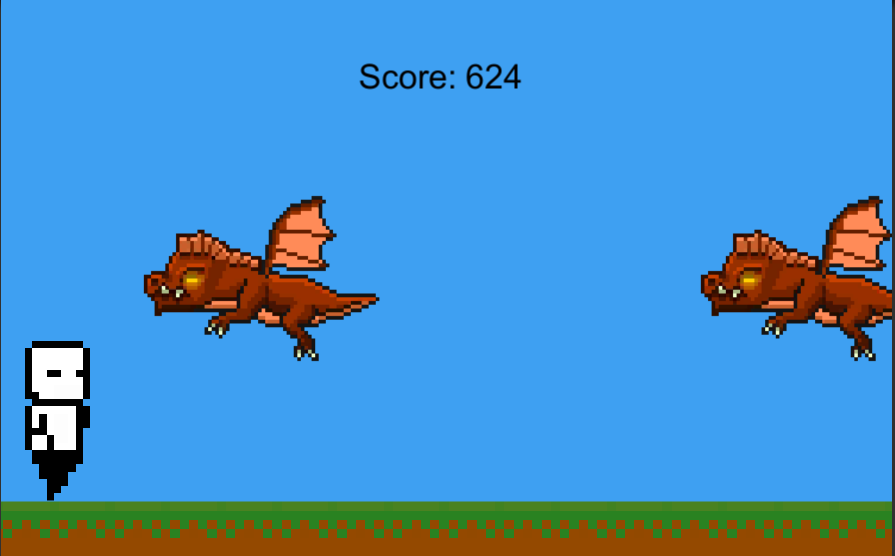
\includegraphics[width=15cm]{game-start}\\
		\caption{Running}
		\label{run}
	\end{figure}
	
	\begin{figure}[h]
		\centering
		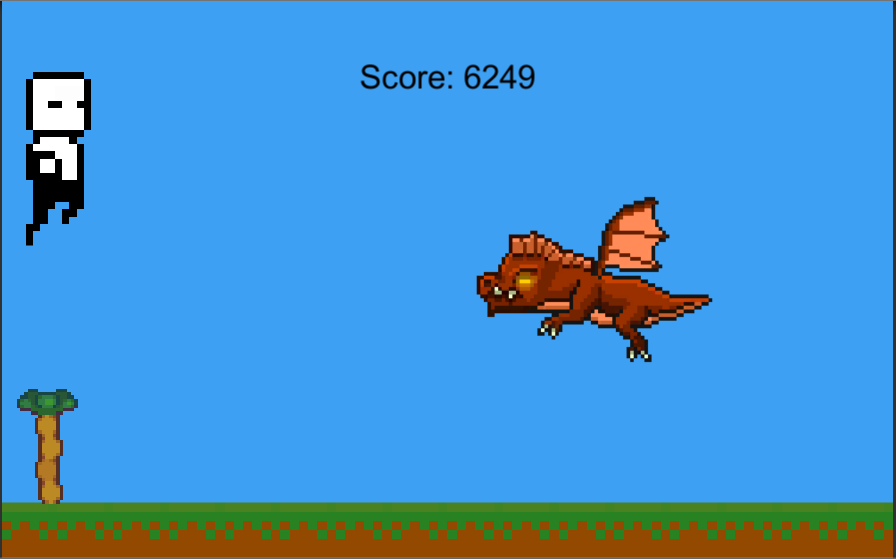
\includegraphics[width=15cm]{Jumping}\\
		\caption{Jumping}
		\label{jump}
	\end{figure}
	
	\begin{figure}[h]
		\centering
		\includegraphics[width=15cm]{Sliding}\\
		\caption{Sliding}
		\label{slide}
	\end{figure}
	
	\begin{figure}[h]
		\centering
		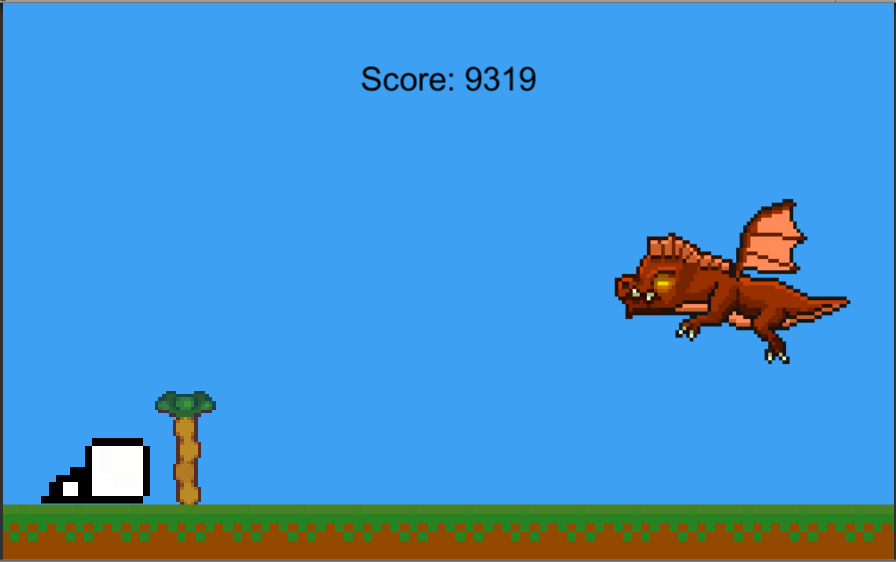
\includegraphics[width=15cm]{GameOver}\\
		\caption{lose}
		\label{lose}
	\end{figure}
\end{center}

\clearpage
